\section{Method}
\label{section:method}

% %   - Introduction
% % In this section we describe the combined isochrone fitting and gyrochronology
% % model implemented in \sd, as well as the inference process.
% % A common approach to stellar age-dating is to make separate age predictions
% % using separate sets of observables.
% % For example, if a star's rotation period, parallax, and apparent magnitudes in
% % a range of bandpasses are available, it is possible to predict its age from
% % both gyrochronology and isochrone fitting separately.
% % How these two age predictions are later combined is then a difficult choice.
% % Is it best to average these predictions, to use the more precise of the two,
% % or the one believed to be more accurate?
% % The methodology described here provides an objective method for combining age
% % estimates.
% % There is, after all, only one age for each star.
% Combining information from different models can be relatively simple as long
% as the processes that generated the data are independent.
% In this case, we are combining observables that relate to the burning of
% hydrogen in the core
% % (this is the process that drives the slow increase in \teff\ and luminosity
% % over time)
% with observables relating to the magnetic braking history of a star (the
% current rotation period)
% and we can assume that, to first order, these two processes are independent.
% % These processes are not truly independent, however any dependence here is
% % unlikely to affect our results within the uncertainties.
% If this assumption is valid, the likelihoods calculated using each model can
% be multiplied together.

Our goal was to infer the age of a star from its observable properties by
estimating the posterior probability density function (PDF) over age,
\begin{equation} \label{eqn:eqn1}
    % p(A|{\bf m_x}, T_{\mathrm{eff}}, \log(g), \hat{F},
    p(A|{\bf m_x}, P_{\mathrm{rot}}, \bar{\omega}),
\end{equation}
where $A$ is age, ${\bf m_x}$ is a vector of
apparent magnitudes in various bandpasses,
% \fhat\ is the {\it observed} bulk metallicity,
\prot\ is the rotation period and \pmega\ is parallax.
Spectroscopic properties (\teff, \logg\ and $\hat{\mathrm{Fe/H}}$) and/or
asteroseismic parameters (\dnu\ and \numax) may also be available for a star,
in which case they would appear to the right of the `$|$' in the above
equation since they are observables.
In order to calculate a posterior PDF over age, other stellar parameters must
be marginalized over.
These parameters are distance ($D$), V-band extinction ($A_V$) and the
inferred metallicity, $F$\footnote{The inferred metallicity is a
model parameter which is different to the {\it observed} metallicity which
would appear on the right side of the $`|'$ in equation \ref{eqn:eqn1}.}.
The final parameter is equivalent evolutionary point (abbreviated to EEP or
$E$), which is a dimensionless number ranging from around 200 for M dwarfs up
to around 500 for subgiants and is 355 for the Sun \citep[see][]{dotter2016,
choi2016}.
Stars are defined as subgiants when their EEP exceeds 454.
Mass is uniquely defined by EEP, age and metallicity.
The marginalization involves integrating over these extra parameters,
\begin{eqnarray} \label{eqn:bayes}
    % & p(A|{\bf m_x}, T_{\mathrm{eff}}, \log(g), \hat{F},
    & p(A|{\bf m_x},
    P_{\mathrm{rot}}, \bar{\omega})
\\ \nonumber
    % & \propto \int p({\bf m_x}, T_{\mathrm{eff}}, \log(g), \hat{F},
    & \propto \int p({\bf m_x},
    P_\mathrm{rot}, \bar{\omega}|
    A, E, F, D, A_V)~p(A)p(E)p(F)p(D)p(A_V)dEdFdDdA_V.
\end{eqnarray}
This equation is a form of Bayes' rule,
\begin{equation} \label{eqn:eqn2}
\mathrm{Posterior} \propto \mathrm{Likelihood} \times \mathrm{Prior},
\end{equation}
where the likelihood of the data given the model is,
\begin{equation} \label{eqn:full_likelihood}
    % p({\bf m_x}, T_{\mathrm{eff}}, \log(g), \hat{F}, \bar{\omega},
    p({\bf m_x}, \bar{\omega}, P_{\mathrm{rot}}|A, E, D, A_V, F),
\end{equation}
and the prior PDF over parameters is,
\begin{equation} \label{eqn:prior}
    p(A)p(E)p(D)p(A_V)p(F).
\end{equation}
The priors we used are described in the appendix.

% %   - Why iso and gyro are independent.
% Not all of the observables on the left of the `$|$' in the likelihood depend
% on all of the parameters to the right of it.
% For example, rotation period, \prot\ does not depend on V-band extinction,
% $A_V$.
% In our model, we make use of conditional independencies like this and use them
% to factorize the likelihood.
% Instead of the likelihood of equation \ref{eqn:full_likelihood},
% where every observable depends on every parameter, our model can be factorized
% as,
% \begin{equation} \label{eqn:factorized}
%     p({\bf m_x}, T_{\mathrm{eff}}, \log(g), \hat{F}, \bar{\omega}
%     |D, A_V, F, A, E) ~p(P_\mathrm{rot}|A, E, F).
% \end{equation}
% where we have introduced two new parameters, $C_{B-V}$, which is the $B-V$
% color that is often used as a mass proxy in the literature and mass itself
% ($M$), which is used in our gyrochronology model to calculate convective
% turnover time and therefore Rossby number.
% The above factorization of the likelihood describes the fact that, in our
% model EEP, age, metallicity, extinction and distance determine the observed
% spectroscopic properties (\teff, \logg, \feh) and apparant magnitudes, ${\bf
% m_x}$) as well as the \cbv\ color and mass of a star.
% In turn, it is a star's age, \cbv\ color, mass and EEP that determine its
% rotation period.
% Breaking up the problem this way allows us to easily combine isochronology and
% gyrochronology and infer the joint age of a star from all its observables.
% While true that rotation period also depends on metallicity at some level, we
% assume that this dependency is weak enough not to significantly affect the
% ages that we infer.

% $C_{B-V}$ and $M$ are not measured but {\it inferred}: they are latent
% parameters.
% We infer $C_{B-V}$ because many stars do not have a directly measured $B-V$
% color.
% For example, most \kepler\ stars have {\it 2MASS} photometry in J, H and K
% bands and \Gaia\ photometry in $G$, $G_{BP}$ and $G_{RP}$, but do not all have
% B and V band colors.
% However, the gyrochronology model we use is calibrated to B-V color, not J-K
% or otherwise \citep{barnes2007, mamajek2008, angus2015}.
% % A probabilistic graphical model (PGM) depicting the joint probability over
% % parameters and observables is shown in figure \ref{fig:PGM}.
% % It describes the conditional dependencies between parameters (in white
% % circles) and observables (in grey circles) with arrows leading from the causal
% % processes to the dependent processes.
% For example, it is the mass, age, metallicity, extinction and distance that
% determines the observed spectroscopic properties (\teff, \logg, \feh)
% and apparant magnitudes, ${\bf m_x}$).
% These parameters also determine the \cbv\ color of a star.
% In turn, it is a star's age and \cbv\ color that determine its rotation
% period.
% Note that, written this way, stellar rotation periods do not directly depend
% on stellar mass.
% Mass, age and metallicity determine $C_{B-V}$, and $C_{B-V}$ along with age
% determines rotation period.
% The purpose of this PGM is not to depict the physical realities of stellar
% evolution, it is only a visual description of the structure of the model we
% use here.
% Breaking up the problem this way allows us to efficiently join isochronology
% and gyrochronology and infer the joint age of a star from all its observables.
% It may well be that rotation period depends directly on mass and metallicity
% in reality, but it is more practical for us to assume that these dependencies
% are weak enough not to significantly affect the ages that we ultimately infer.

%   - The formulas The factorization of the likelihood described in equation
%   \ref{eqn:factorized}
The assumption of independence allowed us to multiply two separate likelihood
functions together: one computed using an isochronal model and one computed
using a gyrochronal model.
We assumed that the probability of observing the measured observables, given
the model parameters was a Gaussian and that the observables were identically
and independently distributed.
The isochronal likelihood function is,
\begin{eqnarray} \label{eqn:isochrones_only_likelihood}
    % & \mathcal{L_{\mathrm{iso}}} = p({\bf m_x}, T_{\mathrm{eff}}, \log(g),
    & \mathcal{L_{\mathrm{iso}}} = p({\bf m_x},
    \bar{\omega}, C_{B-V}|A, E, F, D,
    A_V) \\ \nonumber
    & = \frac{1}{\sqrt{(2\pi)^n \det(\Sigma)}}
    \exp\left( -\frac{1}{2} ({\bf O_I} - {\bf I})^T \Sigma ^{-1}
    ({\bf O_I} - {\bf I})\right),
\end{eqnarray}
where ${\bf O_I}$ is the vector of observables: \pmega, ${\bf m_x}$ plus
spectroscopic and/or asteroseismic observables if available, and $\Sigma$ is
the covariance matrix of that set of observables.
${\bf I}$ is the vector of {\it model} observables that correspond to a set of
parameters: $A$, $E$, $F$, $D$ and $A_V$, calculated using an isochrone model.
We assume there is no covariance between these observables and so this
covariance matrix consists of individual parameter variances along the
diagonal with zeros everywhere else.
The gyrochronal likelihood function is,
\begin{eqnarray} \label{eqn:gyro_likelihood}
    % & \mathcal{L_{\mathrm{gyro}}} = p(P_\mathrm{rot} |A, C_{B-V}, M) \\ \nonumber
    & \mathcal{L_{\mathrm{gyro}}} = p(P_\mathrm{rot} |A, E, F, D, A_V) \\ \nonumber
    & = \frac{1}{\sqrt{(2\pi) \det(\Sigma_P)}}
    \exp\left( -\frac{1}{2} ({\bf P_O} - {\bf P_P})^T \Sigma ^{-1}
    ({\bf P_O} - {\bf P_P})\right),
    % = \prod_i \frac{1}{\sqrt{2\pi}\sigma_i} \exp
    % \left(-\frac{(P_{\mathrm{obs}, i} - P_{\mathrm{pred},
    % i})^2}{2\sigma_i^2}\right),
\end{eqnarray}
% where $P_{\mathrm{obs}, i}$ is the $i$th observed rotation period,
% $P_{\mathrm{pred}, i}$ is the corresponding predicted rotation period,
% calculated from the $i$th age and $C_{B-V}$ values predicted by the isochronal
% model.
where ${\bf P_O}$ is a 1-D vector of observed log-rotation periods, ${\bf
P_P}$ is the vector of corresponding log-rotation periods, predicted by the
model.
$\Sigma_P$ was comprised of individual rotation period measurement
uncertainties, plus an additional variance that was a function of EEP and B-V
color, added in quadrature.
This variance, described in more detail later in this section, accounts for
the stochastic nature of the rotation periods of very hot and very cool stars
and allowed us to predominantly use isochrone fitting to measure the ages of
subgiants.
The full likelihood function used in our model was the product of these two
likelihood functions,
% \begin{eqnarray} \label{eqn:full_likelihood}
%     & \mathcal{L_{\mathrm{full}}} = \frac{1}{\sqrt{(2\pi)^n \det(\Sigma)}}
%     \exp\left( -\frac{1}{2} [{\bf O_I} - {\bf I}]^T \Sigma ^{-1}
%     [{\bf O_I} - {\bf I}]\right) \\ \nonumber
%     & \times
%     \frac{1}{\sqrt{(2\pi) \det(\Sigma_P)}}
%     \exp\left( -\frac{1}{2} [{\bf P_O} - {\bf P_P}]^T \Sigma ^{-1}
%     [{\bf P_O} - {\bf P_P}]\right).
% \end{eqnarray}
\begin{equation}
    \mathcal{L}_{\mathrm{full}} = \mathcal{L}_{\mathrm{iso}} \times
    \mathcal{L}_{\mathrm{gyro}}.
\end{equation}

% Practicalities: sampling, etc.
%-----------------------------------------------------------------------------
%%- isochrones.py
%To calculate ${\bf I}$, the vector of predicted isochronal observables, we
%used the {\tt isochrones.py} {\it python} package which has a range of
%functionalities relating to isochrone fitting.
%The first of the {\tt isochrones.py} functions we used is the likelihood
%function of equation \ref{eqn:isochrones_only_likelihood}.
%The {\tt isochrones.py} likelihood function accepts a dictionary of
%observables which can, but does not {\it have} to include, all of the
%following: \teff, \logg, $F$, parallax and apparent magnitudes in a range of
%colors, as well as the uncertainties on all these observables.
%It then calculates the residual vector $({\bf O_I} - {\bf I})$ where ${\bf
%O_I}$ is the vector of observables and ${\bf I}$ is a vector of corresponding
%predicted observables.
%The prediction is calculated using a set of isochrones \citep[we used the MIST
%models,][]{paxton2011, paxton2013, paxton2015, dotter2016, choi2016,
%paxton2018}, where the set of {\it model} observables that correspond to a set
%of physical parameters is returned.
%This requires interpolation over the model grids since, especially at high
%dimensions, it is unlikely that any set of physical parameters will exactly
%match a precomputed set of isochrones.
%The observables that correspond to a set of physical parameters go into ${\bf
%I}$ and the {\tt isochrones.py} likelihood function returns the result of
%equation \ref{eqn:isochrones_only_likelihood}.
%The second {\tt isochrones.py} function we used is one that predicts \cbv\ for
%a given set of stellar parameters, which was then used to calculate the
%gyrochronal likelihood function of equation \ref{eqn:gyro_likelihood}.

%   - Step-by-step description
The inference processes proceded as follows.
 % (as a reminder, we use {\it
% observables} to refer to the data: \teff, \logg, etc and {\it parameters} to
% refer to the model parameters: EEP, age, metallicity, distance and extinction.
First, a set of parameters: age, EEP, metallicity, distance and extinction,
and observables for a single star were passed to the isochronal likelihood
function in equation \eqref{eqn:isochrones_only_likelihood}.
Then, a set of observables corresponding to those parameters were generated
from the MIST model grid using {\tt isochrones.py} and compared to the
measured observables via the isochronal log-likelihood,
$\ln(\mathcal{L}_{\mathrm{iso}})$.  (also computed using
{\tt isochrones.py}.
The parameters were also passed to the gyrochronology model where $A$, $E$,
$F$, $D$ and $A_V$ were used to calculate $B-V$ color and mass and, in turn,
rotation period.
EEP and $B-V$ were also used to calculate the additional rotation period
variance, added to the individual period uncertainties.
This model rotation period was compared to the measured rotation period using
gyrochronal likelhood function of equation \ref{eqn:gyro_likelihood}.
The gyrochronal log-likelihood was added to the isochronal log-likelihood to
give the full likelihood, which was then added to the log-prior to produce a
single sample from the posterior PDF.

%   - The gyrochronology models
We used the following gyrochronology model to infer ages from rotation
periods,
\begin{equation}
    \log_{10}(P_\mathrm{rot}) \sim \begin{cases}
        % (A^\eta \alpha (B-V - \delta)^\beta, (\sigma_P+f(E, B-V)^2)&, Ro < 2 \\
        \mathcal{N}(\log_{10}(\alpha) + \eta \log_{10}(A) + \beta \log_{10}[B-V
        - \delta], [\sigma_P+f(E, B-V)^2]), & Ro < 2 \\
        \mathcal{N}(\log_{10}(P_\mathrm{max}), [\sigma_P+f(E, B-V)^2]),& Ro \geq 2 \\
        \mathcal{N}(0, [\sigma_P+f(E, B-V)^2]),& B-V < 0.45,
    \end{cases}
\label{eqn:gyro}
\end{equation}
where \prot\ is rotation period in days, $B-V$ is a star's color, $A$ is
stellar age in Myrs, $\sigma_P$ is the logarithmic measured  period
uncertainty and $\eta$, $\alpha$, $\beta$ and $\delta$ took values
0.55, 0.4, 0.31 and 0.45 respectively \citep{angus2015}.
Rotation periods were described as a normal distribution with a power law mean
function for early F and GKM stars with $Ro < 2$, and a constant mean value
for stars with $Ro > 2$ or stars hotter than 0.45 in $B-V$.
The variance of the normal distribution was given by the observational
rotation period uncertainties plus an additional scatter that was a function
of color and EEP (described in more detail later in this section).
The power law functional form was introduced by \citep{barnes2003} and the
parameter values were adopted from the recalibration performed in
\citet{angus2015}, which was based on young cluster stars and old
asteroseismic stars.
Our gyrochronology model reflects the observed ceasing of magnetic braking at
a critical Rossby number of around 2 \citep{vansaders2016}.
The Rossby number, $Ro$, is the ratio of rotation period to convective
overturn time $P_{\mathrm{rot}}/\tau$.
It determines whether a star is still undergoing magnetic braking ($Ro < 2$)
or has stopped spinning down, in which case it retains its terminal rotation
period of $P_\mathrm{max} = 2\tau$ \citep{vansaders2016}.
We estimated the convective overturn time, $\tau$, using equation 11 of
\citet{wright2011}.

The rotation periods of hot stars, cool stars, subgiants and giants evolve
differently to FGK and early M dwarfs.
Stars more massive than around 1.25 M$_\odot$, with a temperature $\gtrsim$
6250 K and a $B-V$ color $\lesssim$ 0.45 do not spin down appreciably over
their main sequence lifetimes because they do not have the deep convective
envelope needed to generate strong magnetic fields.
Late M dwarfs with masses $\lesssim$ 0.3 M$_\odot$, temperatures $\lesssim$
3500 and $B-V$ $\gtrsim$ 1.4 do not start magnetic braking until at least
after the age of Praesepe ($\sim$650 million years).
Both hot and cool stars retain rotation periods that are similar to their
primordial distribution \citep[see \eg][]{matt2012}.
Finally, the rotation periods of evolved stars slow dramatically as their
radii grow.
Although the rotation periods of hot, cool, and evolved stars are less
age-informative than late F, GK and early M dwarfs, they still improve age
measurement precision and accuracy by refining CMD/HRD placement.
We designed a model describing the rotation period variance of these stars,
inflating the variance to high values in regions of parameter space where the
simple gyrochronology power law does not apply or where rotation periods
become stochastic.
% In order to reflect the stochastic rotation periods of hot and cool stars,
% and `switch off' gyrochronology, just using isochrone fitting for
% the hot, cool and evolved stars, we designed a model describing the rotation
% period variance of these stars, inflating the variance to high values in
% regions of parameter space where gyrochronology does not apply.
The variance model was designed to reflect the observed distributions of hot,
cool and evolved stars and naturally reduce the amount of age-information
provided by gyrochronology for stars where the rotation period is
uninformative.
In parts of the CMD/HRD where rotation periods are stochastic, isochronal
information dominates and ages are predominantly inferred via isochrone
fitting.
We used three sigmoid functions to increase the (log) rotation period variance
as a function of $B-V$ and EEP, shown in figure \ref{fig:variance}.
The additional variance was zero where gyrochronology works well: for late F,
GK and early M dwarfs and 0.25 ($\sigma = 0.5$) for hot, cool and evolved
stars.
The logistic functions shown in figure \ref{fig:variance} reach half their
maximum values at 0.45, 1.4 and 454 for hot stars, cool stars and subgiants,
respectively.
The maximum standard deviation value of the logarithmic rotation periods for
all three groups (hot, cool and evolved) was 0.5 and the logistic growth rate,
or steepness, of the three sigmoids were 100, 100 and .2 for hot, cool and
evolved stars respectively.
If a star is both hot and evolved, the additional standard deviation of its
rotation period rises to 1 (no late M dwarfs have yet evolved off the main
sequence so this does not apply to the cool stars).
\begin{figure}
  \caption{
    The additional standard deviation in rotation period added to the
    observational period uncertainties in our model.
    The standard deviation was artificially increased for early F and hotter
    stars ($B-V < 0.45$), late M dwarfs ($B-V > 1.4$) and evolved stars
    (EEP $>$ 454) in order to down-weight the age-information supplied by
    rotation periods and reproduce observed distributions.
    Down-weighting the gyrochronal likelihood by the inverse variance
    ($1/\sigma^2$) allows the ages of these stars to be mostly inferred
    via isochrone fitting.
    The ages of hot and evolved stars can be relatively precisely constrained
    with isochrone fitting since their position on the CMD changes
    rapidly with time, however isochrone fitting cannot constrain the ages of
    late M dwarfs, so the age of any star with $B-V > 1.4$ will not be
    precisely constrained with \sd.
}
  \centering
    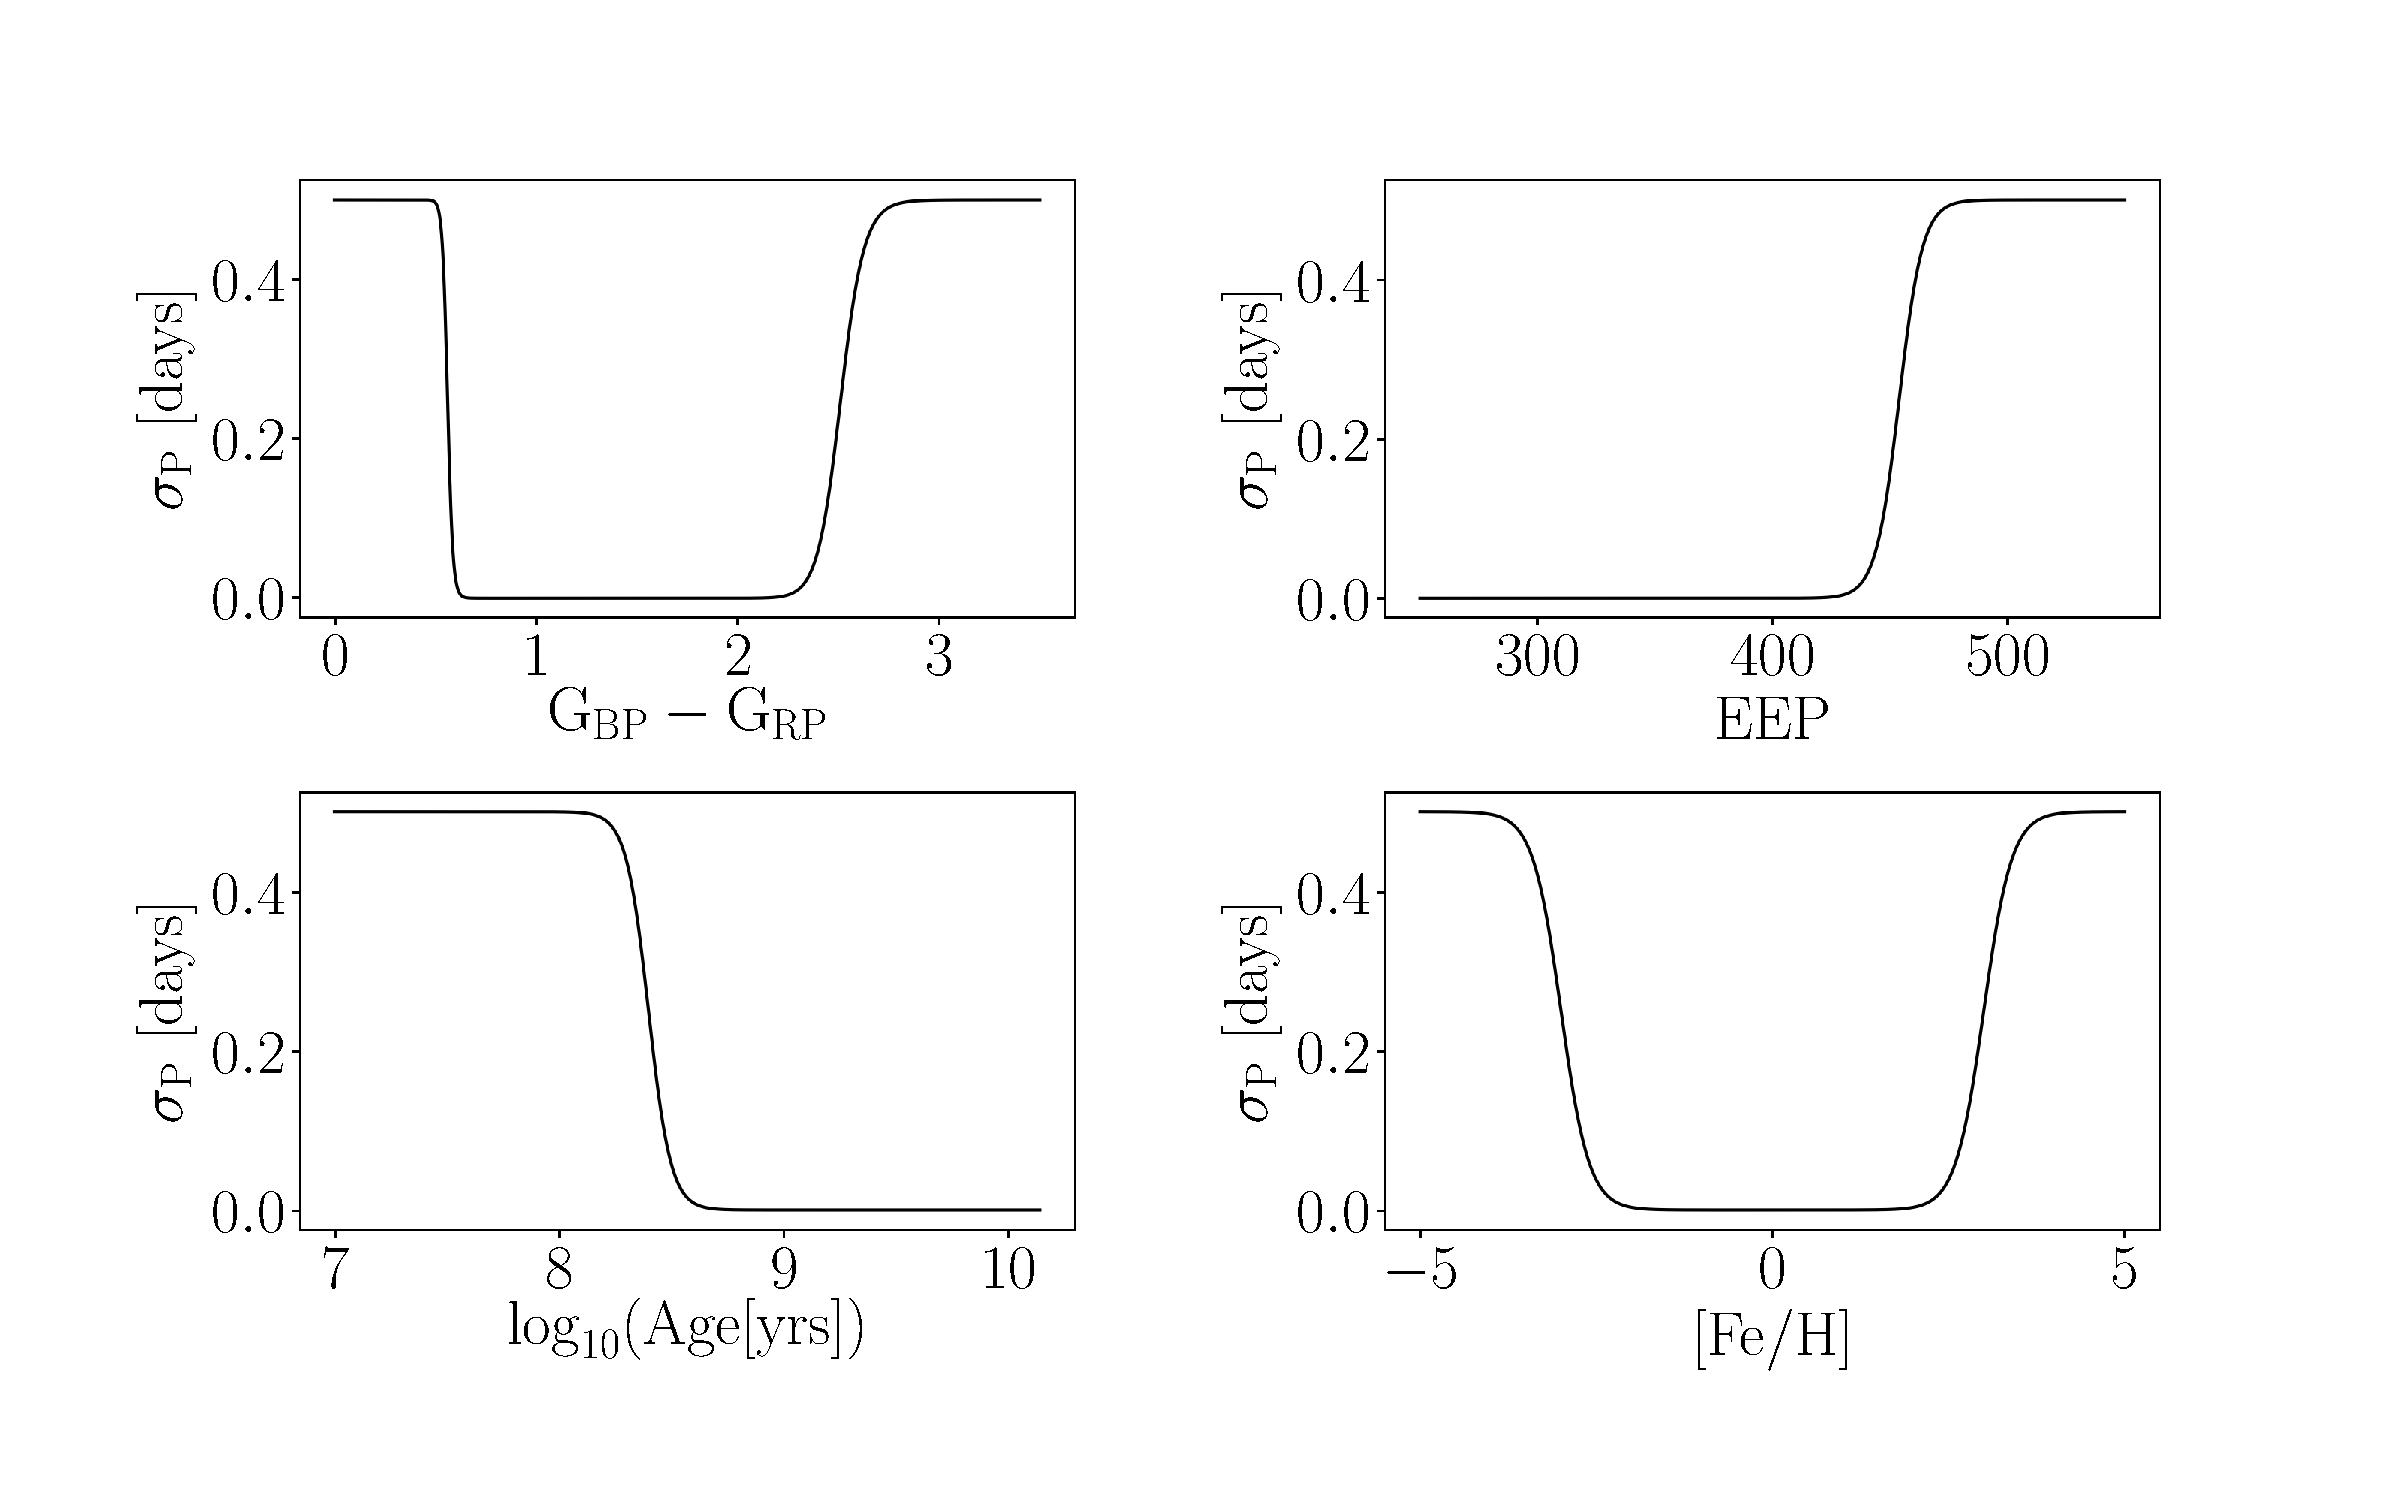
\includegraphics[width=1.\textwidth]{variance}
\label{fig:variance}
\end{figure}
Figure \ref{fig:rotation_model} shows the rotation periods of 841
stars generated from the gyrochronology model.
\begin{figure}
  \caption{
The rotation period model.
Late F, GK and early M dwarfs follow the \citet{angus2015} gyrochronology
    relation (dashed gray lines), with the exception of old, slowly
    rotating stars with large Rossby numbers whose rotation periods are fixed
    at 2$\times$ their convective overturn time.
The rotation periods of early F, late M dwarfs and subgiants were generate
    from a log-normal distribution with standard deviation shown in figure
    \ref{fig:variance}.
The top panel shows the rotation periods vs. B-V colors of simulated stars,
    colored by their age and the bottom panel shows the same stars colored
    by their equivalent evolutionary point (EEP).
    The gray lines describe \citep{angus2015} gyrochrones at ages 1, 3, 5, 7,
    9, 11, and 13 (rotation periods rise with age).
}
  \centering
    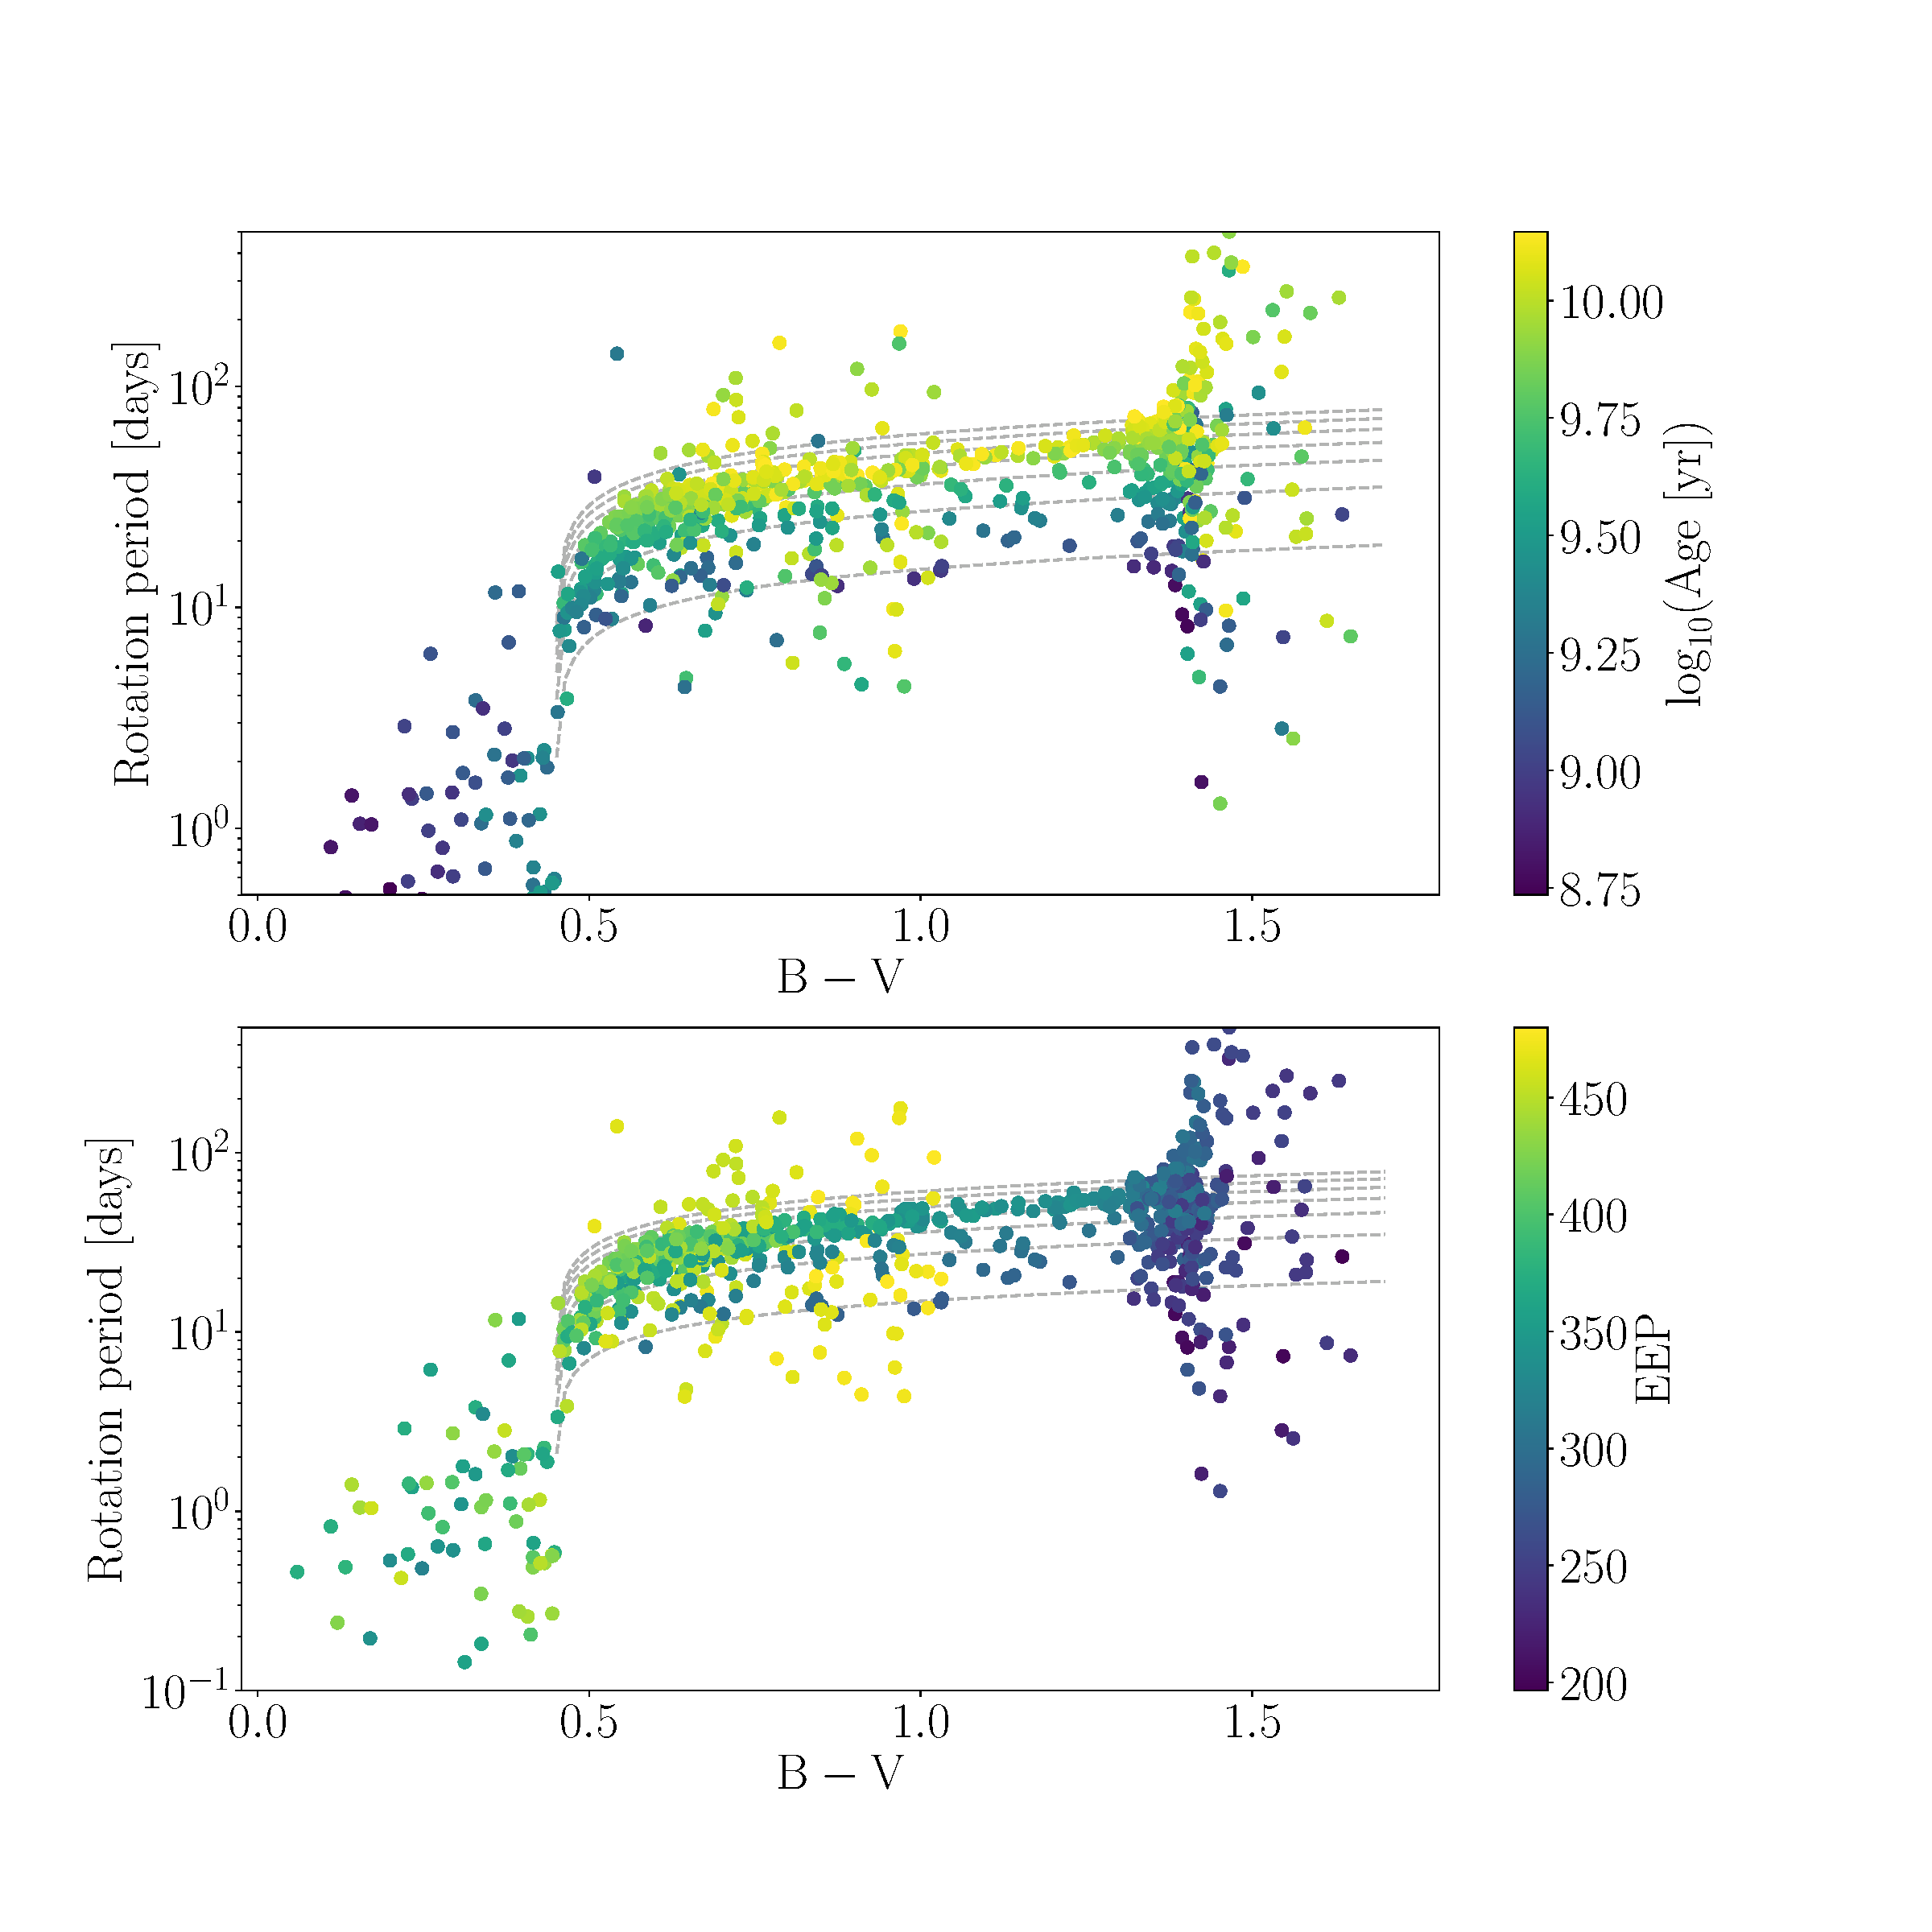
\includegraphics[width=1.\textwidth]{rotation_model}
\label{fig:rotation_model}
\end{figure}

%   - Emcee, including assessing convergence.
We sampled the joint posterior PDF over age, mass, metallicity, distance and
extinction using the affine invariant ensemble sampler, {\tt emcee}
\citep{foreman-mackey2013} with 24 walkers.
Samples were drawn from the posterior PDF until 100 {\it independent} samples
were obtained.
We actively estimated the autocorrelation length, which indicates how many
steps were taken per independent sample, after every 100 steps using the
autocorrelation tool built into {\tt emcee}.
The MCMC concluded when {\it either} 100 times the autocorrelation length was
reached and the change in autocorrelation length over 100 samples was less
than 0.01, {\it or} the maximum of 100,000 samples was obtained.
This method is trivially parallelizable, since the inference process for each
star can be performed on a separate core.
The age of a single star can be inferred in around 10 minutes on a laptop
computer.

% Although the gyrochronology model described above \citep[equation
% \ref{eqn:gyro},][]{angus2015} has been calibrated using a number of cluster
% stars, it does not provide a good fit to any individual cluster.
% No current gyrochronology model is able to capture the behavior of rotation as
% a function of color and age for individual benchmark clusters: the shape of
% this relation is different in each and current models are not flexible enough
% to capture inter-cluster differences in rotational evolution.
% For this reason, we also explored the rotational evolution of a single
% cluster, in order to produce a best-case model and demonstrate the potential
% of rotation-dating in a case where the model is perfectly accurate.
% We chose Praesepe as it is a relatively old open cluster \citep[$\sim$ 600
% Myrs][]{gossage2018}, meaning its Solar-type members have converged onto the
% rotational main sequence, and it is relatively compact on the sky so many of
% its members were observed during a single \ktwo\ campaign.
% In fact, Praesepe was repeatedly observed by \ktwo, in Campaigns 5, 16 and 18,
% however we only use rotation periods published from the analysis of Campaign 5
% in this work \citep{rebull2016}.

% % The Praesepe model
% We used a three-dimensional polynomial model to predict rotation period as a
% function of \gaia\ color and age for Praesepe and the Sun.
% This model consists of a 4th order polynomial in logarithmic Gaia color:
% $G_{Bp} - G_{Rp}$, which we write as $C_G$ for simplicity, and a 1st order
% polynomial (a straight line) in logarithmic age.
% We used \gcolor\ instead of (B-V) because, due to the $\sim$ billion stars
% observed by \gaia, it is now the most abundant and widely available
% photometric color.
% Our gyrochronology likelihood function is designed to compare observed
% rotation period to predicted rotation period.
% For this reason the gyrochronology model we used must predict rotation period
% as a function of age and color.
% However, when {\it calibrating} the gyrochronology model, we chose to make
% {\it age} the dependent variable because the uncertainties on age are much
% greater than the uncertainties on rotation period.
% Since we are using a linear model, the relation is easily invertable.
% We fit the following model to Praesepe members:
% \begin{equation}
%     \log_{10}(A) = a + b\log_{10}(C_G) + c\log_{10}^2(C_G) +
%     d\log_{10}^3(C_G) + e\log_{10}^4(C_G) + f\log_{10}(P)
% \label{eqn:gyro_age_praesepe}
% \end{equation}
% where $P$ is rotation period in days, $C_G$ is Gaia color, $A$ is stellar age
% in years and the lower case letters are free parameters which we fitted to the
% data using linear least squares.
% We adopted an age for Praesepe of 600 million years \citep{gossage2018}, a
% Solar age of 4.56 Gyr \citep{connelly2012}, and a Solar rotation period of 26
% days \citep[][Morris \etal, in prep]{balthasar1986, howe2000}.
% The Sun's color in the Gaia color bandpasses, $G_{Bp} - G_{Rp}$, is 0.82
% \citep{casagrande2018}.
% We found best-fit values: $a = 7.37 \pm 0.03, b = -1.4 \pm 0.1, c = 5.0 \pm
% 0.8, d = -34 \pm 3, e = 66 \pm 14$, and $f = 1.49 \pm 0.02$.
% Rotation periods for Prasepe were obtained from \citet{rebull2017} and their
% \gaia\ colors were obtained by crossmatching their sky-projected positions
% with the \gaia\ DR2 catalog.
% % The $f$ parameter is the inverse of the slope of the rotation period and age
% % which was originally measured to be around 0.5.
% % Our Praesepe and Sun-only fit results in a slightly steeper age dependence of
% % around 0.67, however this value is likely be
% We inverted this relation to predict rotation period as a function of color
% and age,
% \begin{equation}
%     \log_{10}(P) = \frac{\log_{10}(A) - a - b\log_{10}(C_G) - c\log_{10}^2(C_G) -
%     d\log_{10}^3(C_G) - e\log_{10}^4(C_G)}{f}.
% \label{eqn:gyro_age_praesepe}
% \end{equation}
% Both gyrochronology models of equations \ref{eqn:gyro} and
% \ref{eqn:gyro_age_praesepe} are used to predict the ages of individual
% Praesepe stars from their rotation periods and apparent magnitudes in section
% \ref{section:results}.

% % The PGM
% \begin{figure}
%   \caption{
% A probabilistic graphical model (PGM) showing the conditional
% dependencies between the parameters (white nodes) and
% observables (gray nodes) in our model.
% % ${\bf \theta}$ is a vector of {\it parameters}: mass, observed bulk
% %     metallicity, distance and V-band extinction; and ${\bf O}$ is a vector of
% %     {\it observables}: apparent magnitudes, $m_x$, effective temperature,
% %     \teff, surface gravity, \logg, observed bulk metallicity, $\hat{F}$, and
% %     parallax, $\bar{\omega}$.
% % determined by the mass, $M$, age, $A$, distance, $D$, extinction, $A_V$
% % and bulk metallicity, $F$, of a star.
% ${\bf \theta}$ is a vector of {\it parameters}: mass, observed bulk
%     metallicity, distance and V-band extinction; and ${\bf O}$ is a vector of
%     {\it observables}: apparent magnitudes, effective temperature, surface
%     gravity, observed bulk metallicity, and parallax.
%     The observables, ${\bf O}$, are determined by the parameters, $A$ and
%     ${\bf \theta}$.
%     $C_{B-V}$ is a latent parameter that is also determined by the parameters
%     $A$ and ${\bf \theta}$.
%     In our model, the rotation period observable, $P$, is determined {\it
%     only} by the age, $A$, and color ${C_{B-V}}$ parameters.
% The dependencies of observables on parameters and parameters on parameters are
%     indicated by arrows that start at a `parent' node and end at the dependent
%     observable, or `child' node.
% In our model, rotation period does not directly depend on distance,
% extinction, metallicity or mass, only age and B-V color.
% This PGM is a representation of the factorized joint PDF over parameters and
% observables of equation \ref{eqn:factorized}.
% }
%   \centering
%     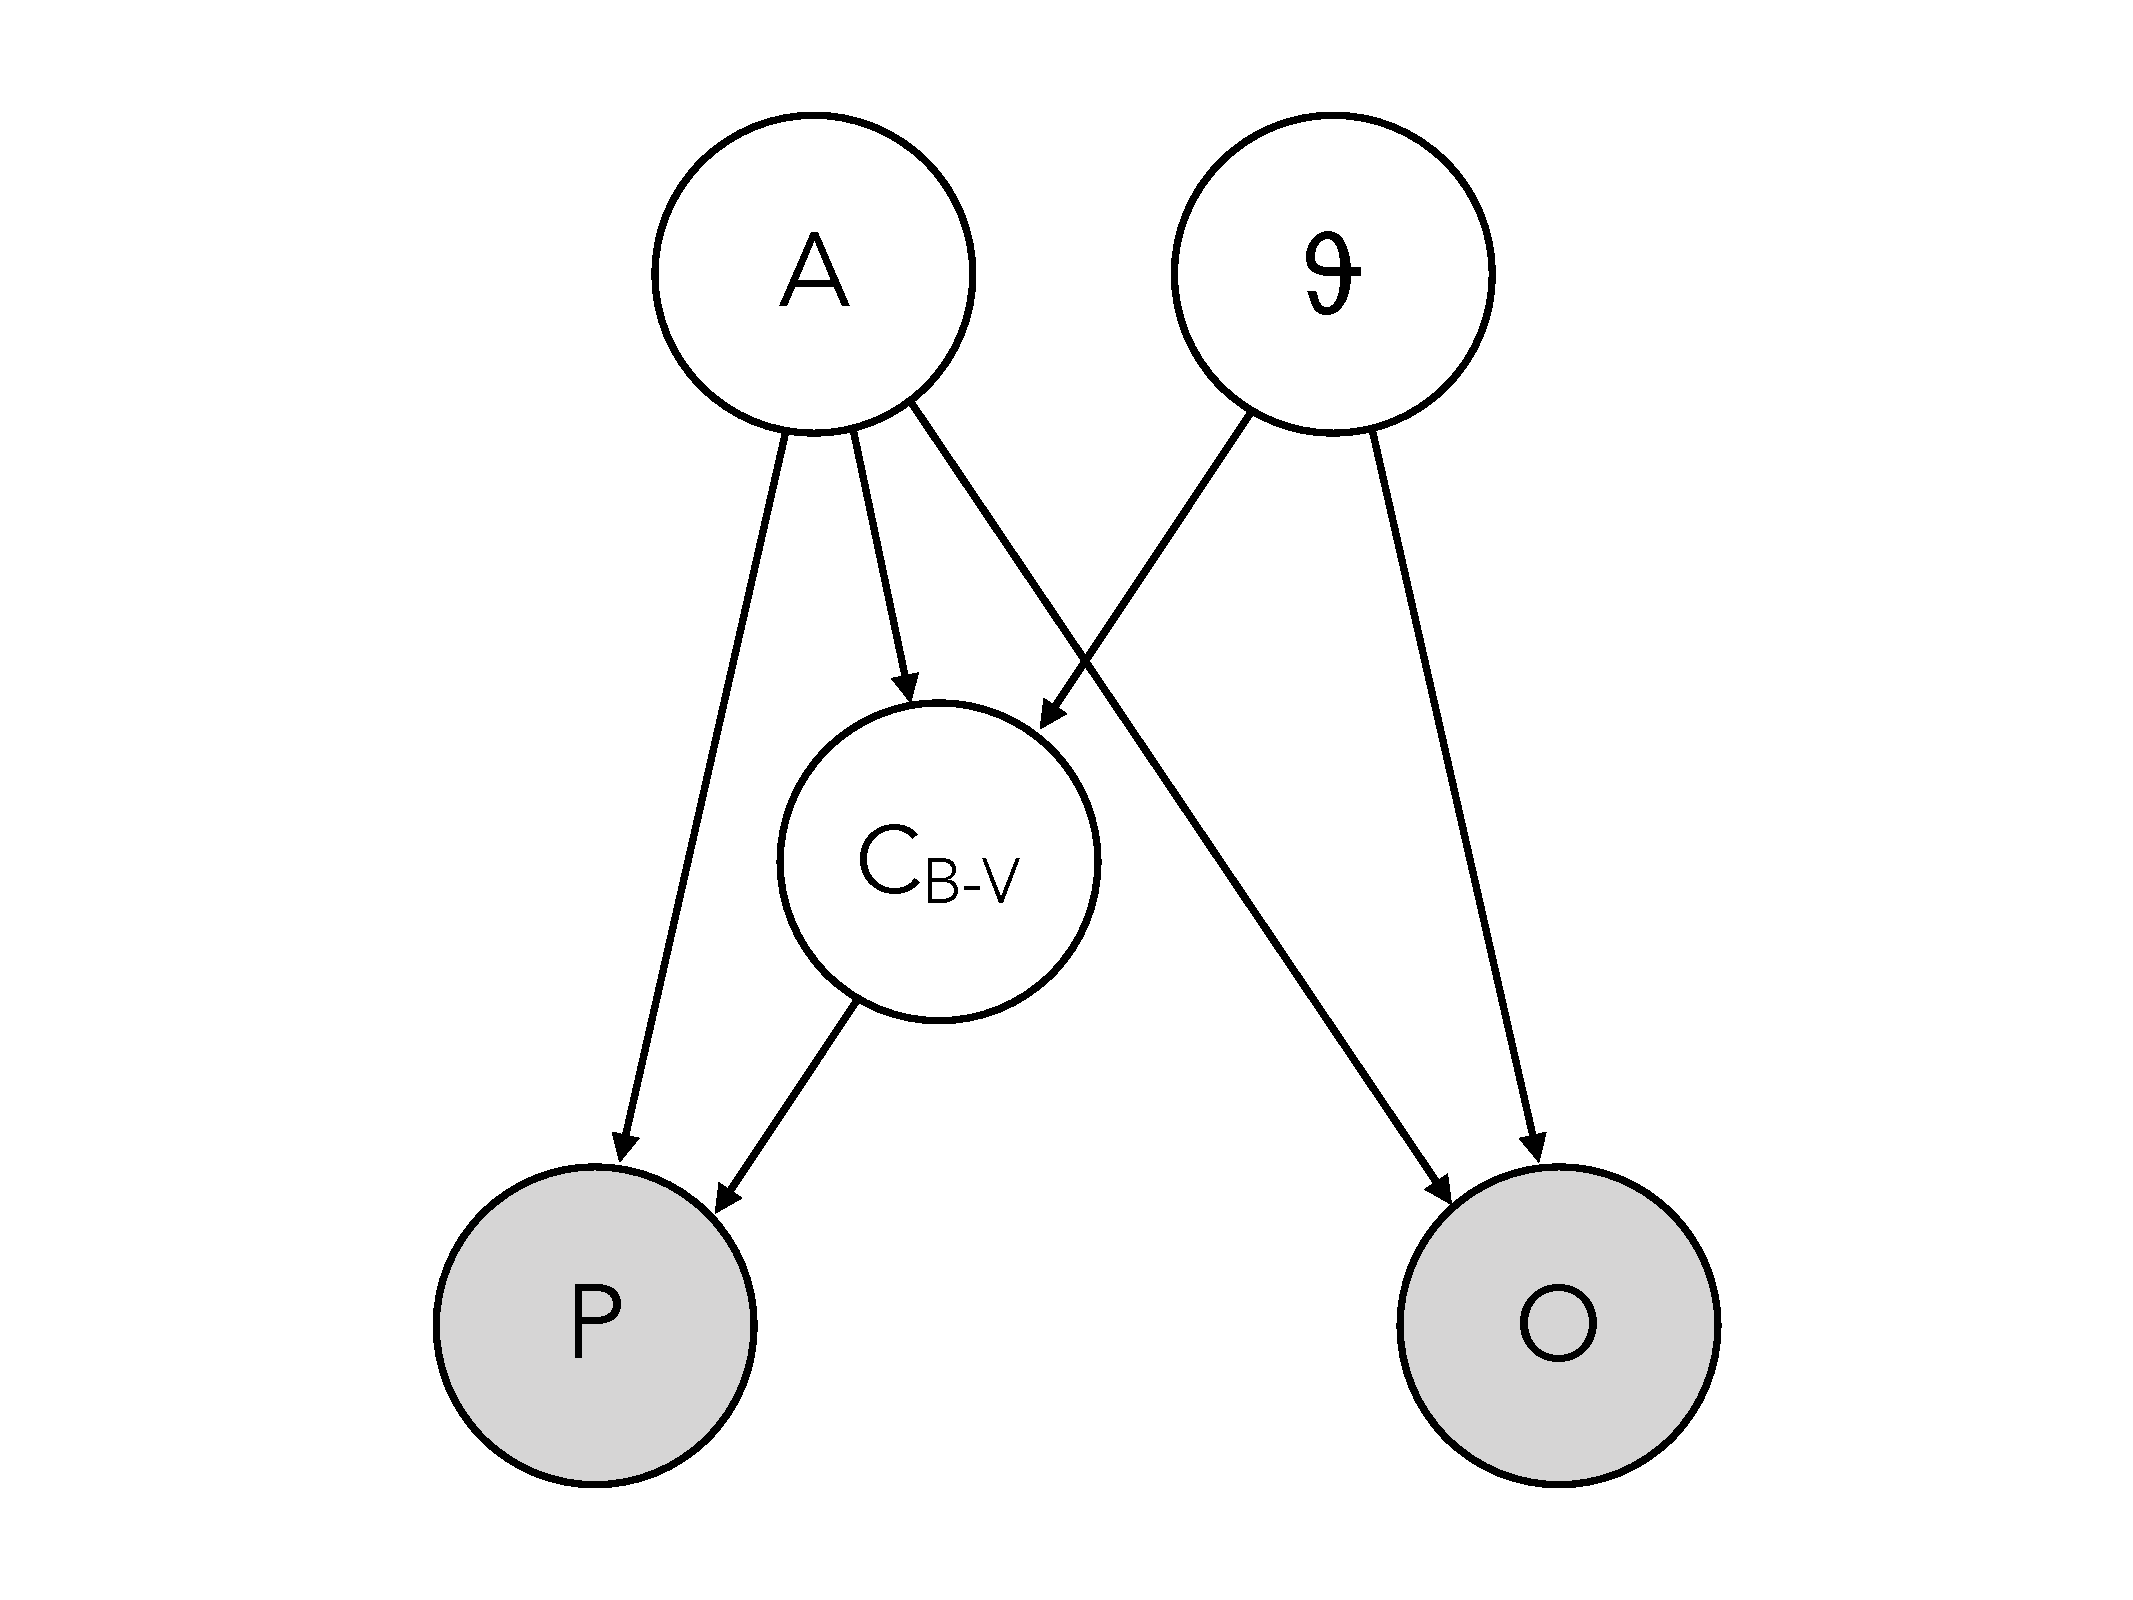
\includegraphics[width=.7\textwidth]{PGM}
% \label{fig:PGM}
% \end{figure}
